\documentclass[letterpaper,12pt]{article}
\usepackage{tabularx} 	% extra features for tabular environment
\usepackage{amsmath}  	% improve math presentation
\usepackage{graphicx} 	% takes care of graphic including machinery
\usepackage{algorithm,algorithmic} 				% describe algorithms
\usepackage[margin=1in,letterpaper]{geometry} 	% decreases margins
\usepackage{cite} 		% takes care of citations
\usepackage{listings} 	% Code writing
\usepackage{pythonhighlight}
\usepackage[final]{hyperref}	% adds hyper links inside the generated pdf file
\hypersetup{
	colorlinks=true,    % false: boxed links; true: colored links
	linkcolor=blue,		% color of internal links
	citecolor=blue,     % color of links to bibliography
	filecolor=magenta,  % color of file links
	urlcolor=blue         
}
\usepackage{blindtext}
%++++++++++++++++++++++++++++++++++++++++


\begin{document}

\title{Intelligent Robot Systems}
\author{Athanasios Manolis (8856), Evangelos Zikopis (8808)}
\date{\today}
\maketitle

\newpage

\begin{abstract}
Report regarding the assignment for the course \textbf{Intelligent Robot Systems}. The general goal is to develop specific modules of an autonomous simulated vehicle that performs full exploration and coverage of an unknown a priori environment.
\end{abstract}

\section{Laser-based obstacle avoidance}

\inputpython{scripts/task_1.py}{0}{50} 

\vspace{2mm} %5mm vertical space

For each of the laser scans, we calculate a value which, essentially, is their effect on the robot's velocity. In order to find the optimal angular velocity, we calculate a positive or negative value, so that the robot goes left or right respectively.

The expression “angle\char`_min+i*angle\char`_increment” is used in order to get the angle transformation of each scan in the interval [-2.094, 2.094], while the trigonometric functions are used to get the appropriate sign. We also divide by $scan[i]^2$ so that we apply the effect of the distance from the obstacle (smaller if it is far or bigger if it is close). The coefficient 0.5 in variable "angular" was selected after tests aiming at smooth changes in the rotational speed of the robot.

Finally, we add the value we found for the linear velocity to 0.3, which we want to be the maximum value. We noticed that if we used a higher value (eg 0.5 or 0.6) then the robot would explore a larger part of the map, but it seemed that in reality it did not have enough time to turn where it should, so it would come very close to obstacles and therefore the speed would of become zero, resulting on an on-site turn. The choice of the value 0.3 seemed to offer the best balance between angular and linear velocity.

\newpage

\section{Path visualization}

\inputpython{scripts/task_2.py}{0}{50}

\vspace{2mm} %2mm vertical space

This task is about visualizing the path’s subgoals on the map. In order to implement it, firstly we multiply each subgoal’s coordinates with the resolution of the map. Secondly, in order to make a translation between the coordinates of the robot pose and the global coordinates of the map we add the robot’s origin to the previous multiplication result. Those two steps are performed for both ‘x’ and ‘y’ coordinates since we have a two-dimensional map. Finally, subgoal’s coordinates are ready to be visualized on the map with a marker.

\section{Path following}

\inputpython{scripts/task_3.py}{0}{50}

\vspace{2mm} %2mm vertical space

This task is about producing the correct velocities for the robot to follow the produced path. The thinking behind our approach is depicted in the next figure and it was based upon the course’s notes.

\newpage

\begin{figure}[!htb]
	\centering
	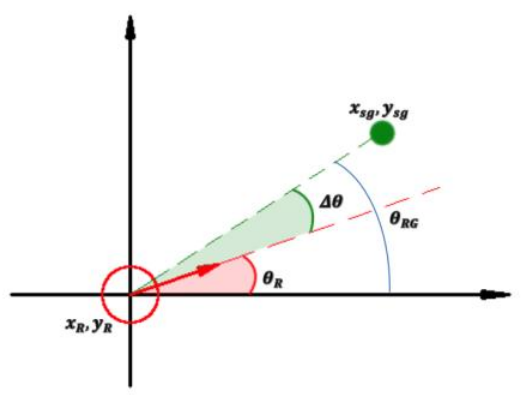
\includegraphics[width=.4\textwidth]{images/angle.png}
	\caption{Angle difference}
	\label{fig:angle}
\end{figure}

The first step of our method calculates the angle difference between the robot’s orientation and the desired sub-target’s position. This angle difference is stored in the variable \textit{dtheta}. The second step concerns the calculation of the robot’s angular (or rotational) speed and it is implemented via an if statement. In this if statement the angular speed is given a value based upon the angle difference between the robot and the sub-target. After the angular speed calculation, the linear speed is given from the formula \[u = ((1-|\omega|)^{20})\cdot0.3\]

The power factor is used to prevent the robot from “overshooting” the desired target.  Finally, both linear and angular speeds are kept in [-0.3, 0.3]

\section{Path following \& obstacle avoidance}

\inputpython{scripts/task_4.py}{0}{50}

\vspace{2mm} %2mm vertical space

We use a motor schema in order to combine velocities from obstacle avoidance and path following procedure. The values of the coefficients c\char`_l and c\char`_a were chosen after experiments. Although, if the linear velocity is 0 (meaning  that there are many obstacles around), then the coefficient for the linear velocity becomes 0 and the coefficient for the angular velocity becomes 1, meaning that the robot will move neither forward nor backwards.

\newpage

\section{Smarter subgoal checking}

\inputpython{scripts/task_5.py}{0}{50}

\vspace{2mm} %2mm vertical space

The main idea of this solution is for the robot to decide to head to a later sub-target, without having to first reach the one that it is trying to reach at the moment. This will happen in 2 cases:
\begin{itemize}
	\item If a later sub-target is closer than the next one, then we make it the next sub-target, and we update the time provided to reach it
	\item If the distance from the next sub-target is less than 5, then we immediately go to the later one, without having to reach it first
\end{itemize}

\newpage

\section{Smart target selection}

\inputpython{scripts/task_6.py}{0}{100}

\vspace{2mm} %2mm vertical space

This task is about finding a smart target selection solution. Our approach aims at covering the full map as fast (and smart) as possible in a Priory Unknown Environments. Our approach is based on the results and novelties presented in \cite{tsardoulias}. The selected method, referred as “minimum cost topological node method” examines and scores every node from the topological graph. If the nodes are more than 25 we take a sample of them, in order to reduce the time wasted in path calculations (more than 1-2 seconds for every node). We construct the path from the robot to every node using A* algorithm. Each nodes’ score is then calculated based on the next weights:

\begin{itemize}
	\item Distance weight (w\char`_dist): The total distance weight is the sum of distances between every sub-path’s neighbor node
	\item Rotation weight (w\char`_rot): The total rotation weight is the sum of the angle difference between the neighbor nodes of the sub-path
	\item Coverage weight (w\char`_cov): Total coverage weight is the sum of coverage value of every node in the sub-path divided by the length of the path
	\item Topological weight (w\char`_topo): The topological weight is representing the presence of obstacles or boundaries near the target. In order to calculate the weight, we examine the brushfire field value of the target and its neighbors. The final value is the mean value of the above
\end{itemize}

After the calculation of the weight values for every node, the values are normalized between 0 and 1. Next, we assign the weights to the cost variables C1-C4. The weights are assigned with a chosen priority. We chose to assign w\char`_topo to C1, since we want our robot to move close to the boundaries of the map. In this way the robot will be moving near the perimeter of the map and the centered free area will be probably covered. This is why we don't select targets located in free areas. Next, w\char`_dist is assigned to C2 since we prefer the robot to catch targets close to its position. Like this we will avoid traversing revisited areas and target selection will be executed more often. At last, w\char`_cov is assigned to C3 and w\char`_rot is assigned to C4. Next, a priority weight (C\char`_PW) and a smoothing factor (C\char`_SF) are calculated based on the values of C1-C4 for every node. The final priority for every node is calculated as C\char`_FP = C\char`_PW*C\char`_SF. The node with the lowest final priority is selected as the next target.

In figures \ref{fig:random_target} and \ref{fig:smart_target} shown below, we can notice that the smart target approach is much better than the random one. The total time elapsed in order to get the same map coverage result may be similar in both methods. However ,it is clear that in the smart selection method the total distance traversed is way smaller.

\begin{figure}[!htb]
	\centering
	\begin{minipage}[b]{0.45\textwidth}
		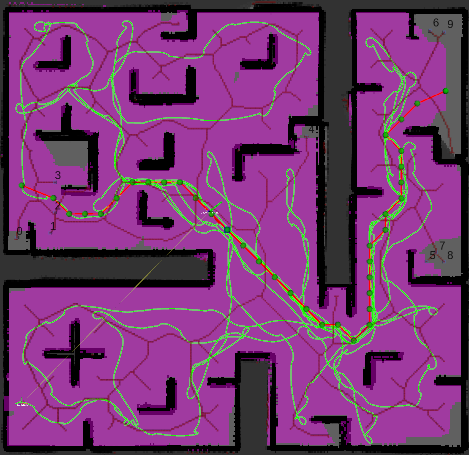
\includegraphics[width=\textwidth]{images/random_target.png}
		\caption{Random target selection}
		\label{fig:random_target}
	\end{minipage}
	\hfill
	\begin{minipage}[b]{0.45\textwidth}
		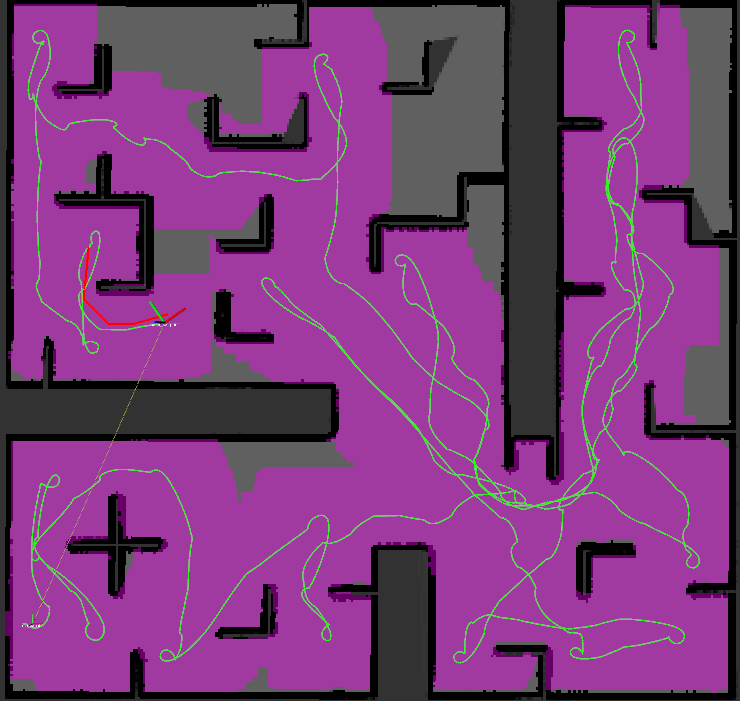
\includegraphics[width=\textwidth]{images/smart_target.png}
		\caption{Smart target selection}
		\label{fig:smart_target}
	\end{minipage}
\end{figure}

\section{Path optimization / alteration}

\inputpython{scripts/task_extra1.py}{0}{100}

\vspace{2mm} %2mm vertical space

In this task, we follow the method indicated at lecture 9 (also linked to the recommended Udacity course on AI in Robotics). Y represents the new, smoothed path, while X represents original path. In each iteration we minimize:

\begin{itemize}
	\item the distance between the coordinates of the original path and the smoothed path
	\item the difference between the coordinates of the smoothed path at time step i, and neighboring time steps
\end{itemize}

In order to minimize all these values simultaneously, we use Gradient Ascent. We adjust the importance of the smoothing of y\char`_i with respect to the un-smoothed trajectory by the weight 'a', and the importance of the smoothing of y\char`_i with respect to neighboring smoothed coordinates, by the weight 'b'.

The iterations will keep going, only while the change to be done has a value of at least 0.0001.


%++++++++++++++++++++++++++++++++++++++++
% References section will be created automatically 
% with inclusion of "thebibliography" environment
% as it shown below. See text starting with line
% \begin{thebibliography}{99}
% Note: with this approach it is YOUR responsibility to put them in order
% of appearance.

\newpage

\begin{thebibliography}{99}
	
	\bibitem{tsardoulias}
	Tsardoulias, E.G., Iliakopoulou, A., Kargakos, A. et al. Cost-Based Target Selection Techniques Towards Full Space Exploration and Coverage for USAR Applications in a Priori Unknown Environments. J Intell Robot Syst 87, 313–340 (2017)
	
	%\bibitem{tutorialspoint} \emph{Polygon Filling Algorithms},  available at \\
	%\texttt{https://www.tutorialspoint.com/computer\_graphics/polygon\_filling\_algorithm.htm}
	
\end{thebibliography}



\end{document}
